{The figure shows the graphs of $f$, $\fp$, $\fpp$ and $\fpp'$. Identify each curve and explain your choices.\\
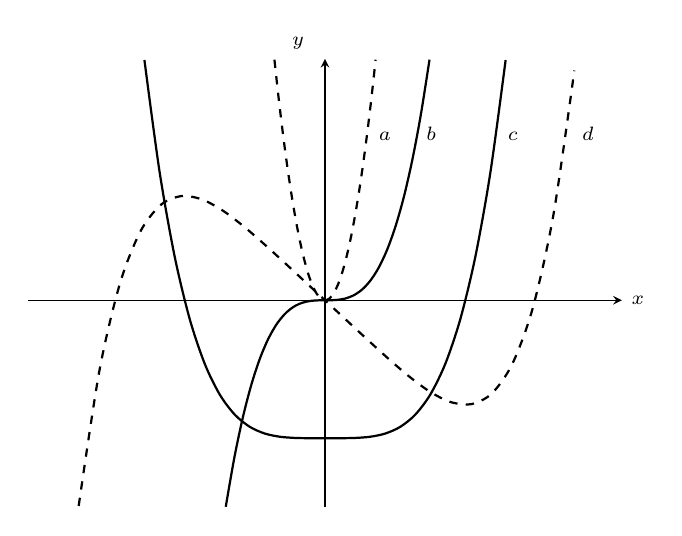
\begin{tikzpicture}
 \begin{axis}[xtick=\empty, ytick=\empty, axis y line=middle,axis x line=middle,
   ymin=-3,ymax=3.5, xmin=-2,xmax=2, name=myplot, xscale=1.1/1,]

  \addplot [{\colorone}, dashed, smooth, domain=-1.66:1.68,thick] {.5*x^5-2*x}; 
  \node[label={30:{\scriptsize $d$}}] at (axis cs:1.6,2.1) {};

  \addplot [{\colortwo}, smooth, domain=-1.217:1.217,thick] {2.5*x^4-2};
  \node[label={30:{\scriptsize $c$}}] at (axis cs:1.1,2.1) {};

  \addplot [{\colorone}, smooth, domain=-.669:.704, thick] {10*x^3};
  \node[label={30:{\scriptsize $b$}}] at (axis cs:.55,2.1) {};

  \addplot [{\colortwo}, dashed, smooth, domain=-.341:.341, thick] {30*x^2};
  \node[label={30:{\scriptsize $a$}}] at (axis cs:.23,2.1) {};

 \end{axis}
 \node [right] at (myplot.right of origin) {\scriptsize $x$};
 \node [above] at (myplot.above origin) {\scriptsize $y$};
\end{tikzpicture}}
{$d$ is $f$, $c$ is $\fp$, $b$ is $\fpp$, and $a$ is $\fpp'$}
